\documentclass{article}
\usepackage[T1]{fontenc}
\usepackage{lmodern}
\usepackage{graphicx}
\usepackage{amsmath,amssymb}
\usepackage[a4paper,margin=2cm]{geometry}
\usepackage[absolute,overlay]{textpos}
\setlength{\TPHorizModule}{1mm}
\setlength{\TPVertModule}{1mm}
\usepackage[indonesian]{babel}
\usepackage{hyperref}
\setlength{\emergencystretch}{2em}
% unit: Halaman 37

\begin{document}

% === Halaman 37 (llm) ===

\vspace{141.37mm}

Beberapa algoritma kriptografi simetri:
\vspace{5mm}

% deskripsi: Tabel perbandingan beberapa algoritma kriptografi simetri yang mencakup kolom Cipher, Pembuat, Panjang Kunci, dan Keterangan.
% bbox normalisasi: [0.0700, 0.2380, 0.8890, 0.7140]
\begin{textblock*}{171.99mm}(14.70mm,70.69mm)
\noindent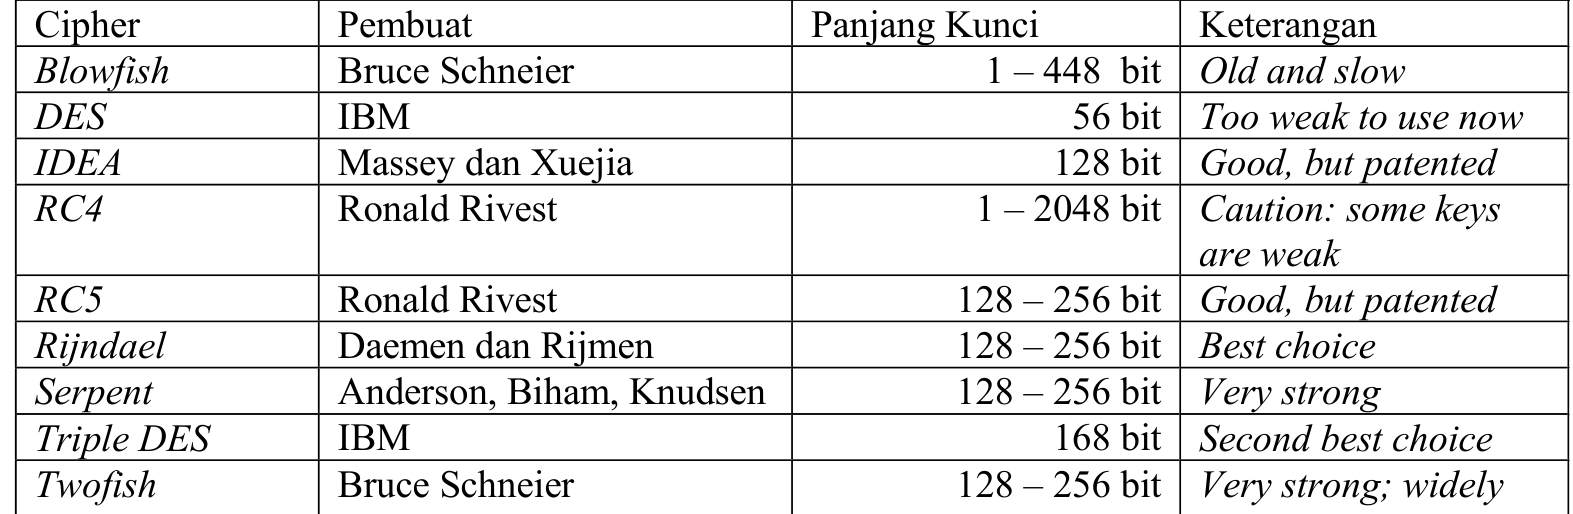
\includegraphics[width=171.99mm,height=141.37mm]{../../images/llm/page_037_img_01.png}%
\end{textblock*}

\end{document}
